\documentclass[smaller ,table,usenames,dvipsnames]{beamer}
\usepackage{xcolor}
\usepackage{bbm}

%\usepackage{beamerthemesplit}
%\usepackage{xmpmulti}
\usepackage{subcaption}

\usetheme{Boadilla}
%\usetheme{Goettingen}
%\usepackage{sansmathaccent}
\pdfmapfile{+sansmathaccent.map}
\usepackage{amsmath}
\usepackage{graphicx}
\usepackage{booktabs}
\usepackage{tabularx}
\usepackage{lipsum}
\usepackage{epstopdf}

\usepackage{url}
\usepackage{graphicx}
\usepackage{epstopdf}
\usepackage{graphics}
\usepackage{rotating}
% \usepackage{color}
\usepackage{framed}
\usepackage{qtree}
\usepackage{amsmath}
\usepackage{wrapfig }
\usepackage{slashed}
\usepackage{ulem}
\usepackage{cancel}
\usepackage{booktabs}

\usepackage{multicol}
\usepackage{etex}
%\usepackage{vwcol}

\usepackage{tabularx}
\usepackage{natbib}
\usepackage{xcolor}
\usepackage{multirow}
% \usepackage{multicol}


\setbeamertemplate{theorems}[numbered]
\definecolor{green}{HTML}{66FF66}
\definecolor{myGreen}{HTML}{009900}

\renewcommand{\familydefault}{\sfdefault}
\renewcommand{\arraystretch}{1.5}

\newcommand{\D}{\mathbf{d}}
\newcommand{\barq}{\bar{Q}}
\newcommand{\qasq}{\quad \mbox{as} \quad}
\newcommand\HUGE[1]{{\sf\fontsize{24}{24}\selectfont \textcolor{blue}{\textbf{#1}}}}
\newcommand\BIG[1]{{\sf\fontsize{16}{16}\selectfont #1}}
\newcommand{\Pro}{\mathbb{P}}
\newcommand{\E}{\mathbb{E}}
\newcommand{\var}{\text{Var}}
\newcommand{\cov}{\text{Cov}}
\newcommand{\condis}{\stackrel{\mathcal{D}}{\longrightarrow}}
\newcommand{\eqdis}{\stackrel{\mathcal{D}}{=}}
\newcommand{\neqdis}{\stackrel{\mathcal{D}}{\neq}}
\newcommand{\ngo}{\stackrel{n\hspace{.05cm}\uparrow \infty}{\longrightarrow}}
\newcommand{\hgo}{\stackrel{h\hspace{.05cm}\downarrow 0}{\longrightarrow}}
\newcommand{\?}{\stackrel{?}{=}}
\newcommand{\iidsim}{\stackrel{I.I.D}{\sim}}
\newcommand{\ind}{\perp\!\!\!\!\perp}
\newcommand{\cL}{\mathcal{L}}
\newcommand{\cc}{\mathcal{C}}
\newcommand{\inS}{\in\mathcal{S}}
\newcommand{\bpi}{\boldsymbol{\pi}}
\newcommand{\blmd}{\boldsymbol{\lambda}}
\newcommand{\blmdz}{\boldsymbol{\lambda}^{(0)}}
\newcommand{\bmP}{\mathbf{P}}
\newcommand{\lmdz}{\lambda^{(0)}}
\newcommand{\bmu}{\boldsymbol{\mu}}
\newcommand{\bP}{\boldsymbol{P}}
\newcommand{\bQ}{\boldsymbol{Q}}
\newcommand{\bR}{\boldsymbol{R}}
\newcommand{\bS}{\boldsymbol{S}}
\newcommand{\bB}{\boldsymbol{B}}
\newcommand{\bI}{\boldsymbol{I}}
\newcommand{\bn}{\boldsymbol{n}}
\newcommand{\be}{\boldsymbol{e}}
\newcommand{\balpha}{\boldsymbol{\alpha}}
\newcommand{\clr}{\mathcal{R}}
\newtheorem{proposition}[theorem]{Proposition}
\newcommand*{\rom}[1]{\expandafter\@slowromancap\romannumeral #1@}
\newcommand{\RR}{\mathbb{R}}
\newcommand{\bluetext}[1]{\textit{\textcolor{blue}{#1}}}
%\captionsetup[figure]{labelformat=empty}% redefines the caption setup of the figures environment in the beamer class.
\newcommand{\barn}{\bar{N}}
\usepackage{tikz}
\usetikzlibrary{fadings,shapes.arrows,shadows}

\tikzfading[name=arrowfading, top color=transparent!0, bottom color=transparent!95]
\tikzset{arrowfill/.style={top color=red!20, bottom color=red, general shadow={fill=black, shadow yshift=-0.8ex, path fading=arrowfading}}}
\tikzset{arrowstyle/.style={draw=red,arrowfill, single arrow,minimum height=#1, single arrow,
		single arrow head extend=.4cm,}}
\newcommand{\tikzfancyarrow}[2][2cm]{\tikz[baseline=-0.5ex]\node [arrowstyle=#1] {#2};}

%\usepackage{enumitem}

%% Command to fill out the end of a page
\newcommand{\dofill}{\vspace\fill}
\newcommand\oldvspace[1]{}

%% Command to generate model frame
\newcommand\makemodel[8]{
    {\small
%   \begin{tabular}{p{1.7cm}p{0.6cm}p{1.6cm}p{0.6cm}p{0.5cm}p{0.9cm}p{1.5cm}}
    \begin{tabular}{lllllll}
    \HUGE{#1} & \HUGE{/} & \HUGE{#2} & \HUGE{/} & \HUGE{#3} & \HUGE{#4} & \HUGE{#5}\bigskip\\
    \multicolumn{2}{l}{\parbox{2.2cm}{#6}} &
    \multicolumn{3}{l}{\parbox{2.2cm}{#7}} &
    \multicolumn{2}{r}{\parbox{2cm}{\raggedleft #8}} \bigskip\\
    \end{tabular}}
    }

\newcommand\makemodelsimple[5]{
    {\small
%   \begin{tabular}{p{1.7cm}p{0.6cm}p{1.6cm}p{0.6cm}p{0.5cm}p{0.9cm}p{1.5cm}}
    \begin{tabular}{lllll}
    \HUGE{#1} & \HUGE{/} & \HUGE{#2} & \HUGE{/} & \HUGE{#3} \bigskip\\
    \multicolumn{2}{l}{\parbox{2.2cm}{#4}} &
    \multicolumn{2}{l}{\parbox{2.2cm}{#5}}
    \end{tabular}}
    }



\setbeamerfont{frametitle}{size=\large}
%\setbeamertemplate{itemize items}[ball]
%\setbeamertemplate{itemize items}[default]
\setbeamertemplate{itemize items}[triangle]
%\setbeamertemplate{itemize items}[circle]
%\setbeamertemplate{itemize items}[square]


%\setbeamertemplate{bibliography item}
\bibliographystyle{plainnat}


\label{Begin Document}
\begin{document}



%\title[Optimal Control to Production System]{\Large{Optimal Control to a Production System with Time-Varying Demand}}\\
%\author[Ling Zhang]{\textcolor{blue}{\large Ling Zhang\inst{1}, Chihoon Lee \inst{2}, Xin Liu\inst{3}, Yunan Liu \inst{1}}}
%%\institute[NC State University]{Department of Industrial and Systems Engineering\\ NC State University}
%\institute[NCSU ISE]{\inst{1} Department of Industrial and Systems Engineering, North Carolina State University, Raleigh, NC 27695 \and
%	\inst{2} School of Business, Stevens Institute of Technology, Hoboken, NJ 07030 \and
%	\inst{3} Department of Mathematical Sciences, Clemson University, Clemson, SC 29634}
%\date{}


\title[Dynamic Patient Scheduling in ED]{\Large{Dynamic Patient Scheduling in ED\\ A Tandem Queueing Model with Time-Varying Arrivals}}
\author[Ling Zhang]{\textcolor{purple}{\large Ling Zhang}\\ Joint work with Nilay Tanik Argon\inst{1}, Serhan Ziya\inst{1} and Yunan Liu\inst{2}}

\institute[NC State]{
\inst{1} Department of Statistics and Operations Research, UNC \and
\inst{2} Department of Industrial and Systems Engineering, NC State University 
}

\date{\today}


\frame{
    \titlepage
}

\section{Background}
\begin{frame}{Background: Congested ER ``Code Black''}
\begin{figure}[htp]
	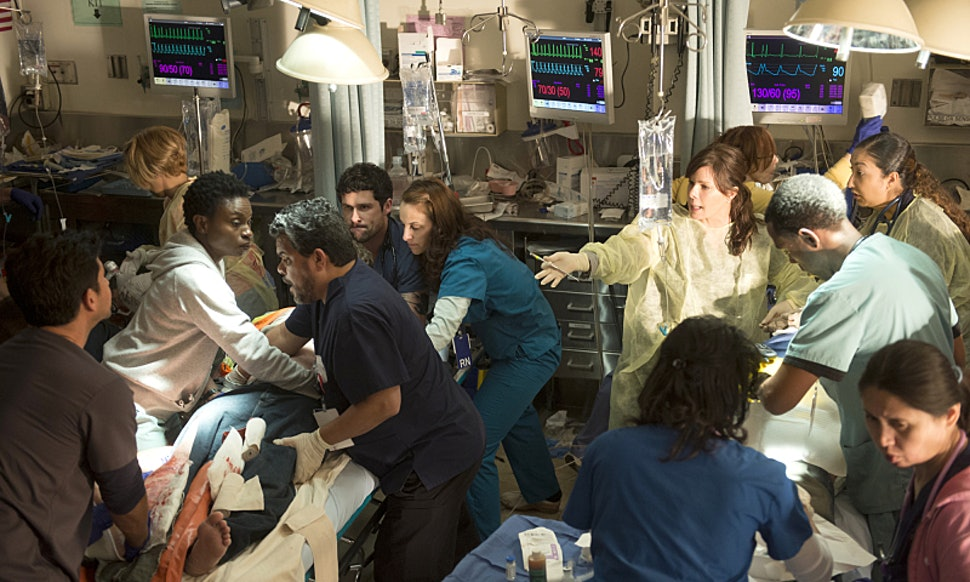
\includegraphics[width=0.85\linewidth]{./Figures/ER_codeblack}
	\caption*{Overcrowded ER leads to misdiagnose and delay in treatment. }
\end{figure}
\vspace{-0.1in}
\begin{itemize}
    \item We want to focus on: time-varying, delay, and strategic nurse staffing.
\end{itemize}
\end{frame}

\begin{frame}{Background: Time-varying Demand}
    \begin{figure}
        \centering
        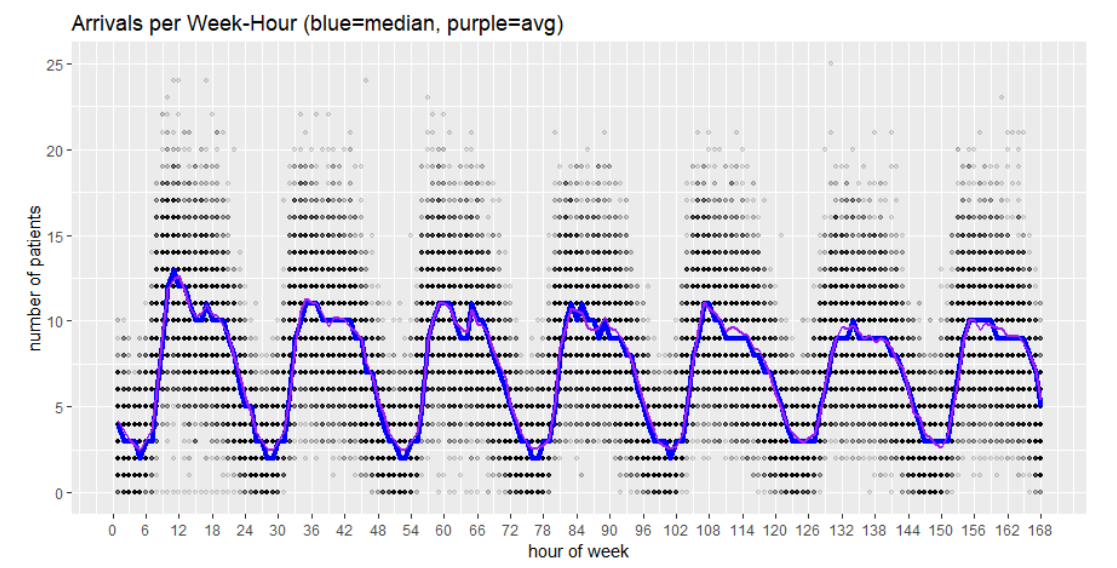
\includegraphics[width=0.9\textwidth]{./Figures/ED_demand}
        \caption*{Time-varying demand to ED: real data in an NC hospital}
        \label{fig:time_varying_demand}
    \end{figure}
    
\end{frame}

% \begin{frame}{Background: Multiple Nurse Duties/ Insufficient Amount of Nurses}
%     \begin{figure}
%         \centering
%         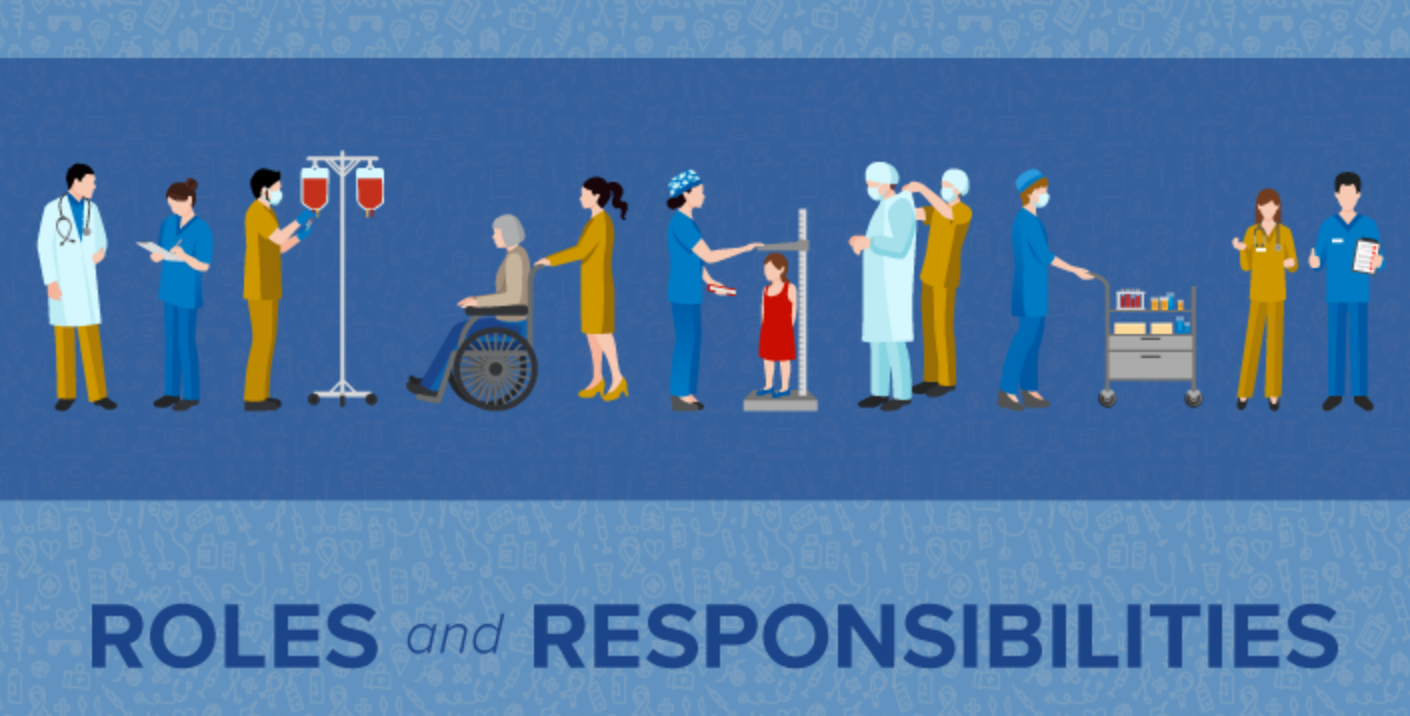
\includegraphics[width=0.8\textwidth]{./Figures/nurse_duties}
%         \caption{Multiple duties of a ED nurse: triage, basic treatment, etc}
%         \label{fig:nurse_duties}
%     \end{figure}
% Question: when the ED is congested, how to staff nurses/prioritize patients?
% \end{frame}

\begin{frame}{Background: Insufficient Amount of Nurses}
\begin{figure}
    \centering
    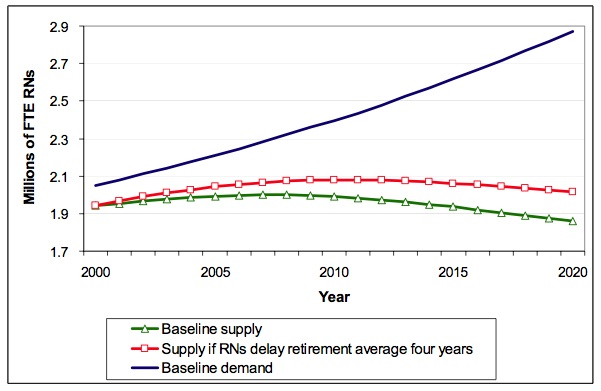
\includegraphics[width=0.8\textwidth]{./Figures/not_enough_nurses}
    % \caption{Supply and Demand Forecast \cite{aiken2002hospital} }
    \label{fig:not_enough_nurses}
\end{figure}

\vspace{-0.2in}
\begin{itemize}
    \item Challenges:
    \begin{itemize}
        \item periods of overloading and underloading
        \item how to strategically staff nurses
    \end{itemize}
\end{itemize}
\end{frame}

% \begin{frame}{Background: Multiple Nurse Duties/ Insufficient Amount of Nurses}
% \begin{figure}
%     \centering
%     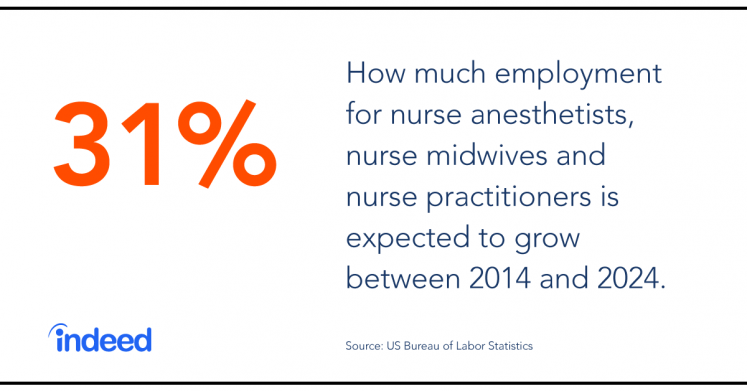
\includegraphics[width=0.8\textwidth]{./Figures/nurse_demand}
%     \caption{Report from indeed.com}
%     \label{fig:nurse_demand}
% \end{figure}    

% \textcolor{black}{Question we want to answer}
% \begin{itemize}
%     \item \textcolor{Cyan}{How to strategically staff limited nurse resources and prioritize patients?}
% \end{itemize}
% \end{frame}

\section{Research Statement}
\begin{frame}{Research Problem}
% Model an elementary component in a ED: a t.\\
An elementary component: \textcolor{Cyan}{a two-phase treatment with delay}
\smallskip
\begin{itemize}
    \item Patient arrival follows NHPP with rate \textcolor{Cyan}{$\lambda(t)$} at phase 1.\medskip
	\item Phase 1 treatment: \textcolor{Cyan}{exp. with rate $\mu_1$}. \medskip 
	\item An \textcolor{Cyan}{$\alpha$} proportion of patients need further treatment. \medskip
	\item Delay: blood work, waiting for test results, etc: \textcolor{Cyan}{exp. delay with rate $\mu_d$}.\medskip
	\item Phase 2 treatment: \textcolor{Cyan}{exp. with rate $\mu_2$} .\medskip
\end{itemize}
A challenge:\smallskip
\begin{itemize}
	\item {Limited number of nurses or beds}: \textcolor{Cyan}{$s_1(t) + s_2(t) \leq C$}.\medskip
\end{itemize}

Question:
\begin{itemize}
	\item How to design a scheduling policy to minimize 
	\begin{itemize}
	   % \item time-varying queue length: \textcolor{Cyan}{$\int Q_1(t)+Q_2(t)dt$}
	    \item weighted queue length: \textcolor{Cyan}{$\int c_1Q_1(t)+c_2Q_2(t)dt$}
	\end{itemize}
% 	such that waiting queues at both stations are minimized?
\end{itemize}
\end{frame}


\begin{frame}{A Tandem Queueing Network Model: A Many-server Model}
	\begin{figure}[h!]
	\centering
	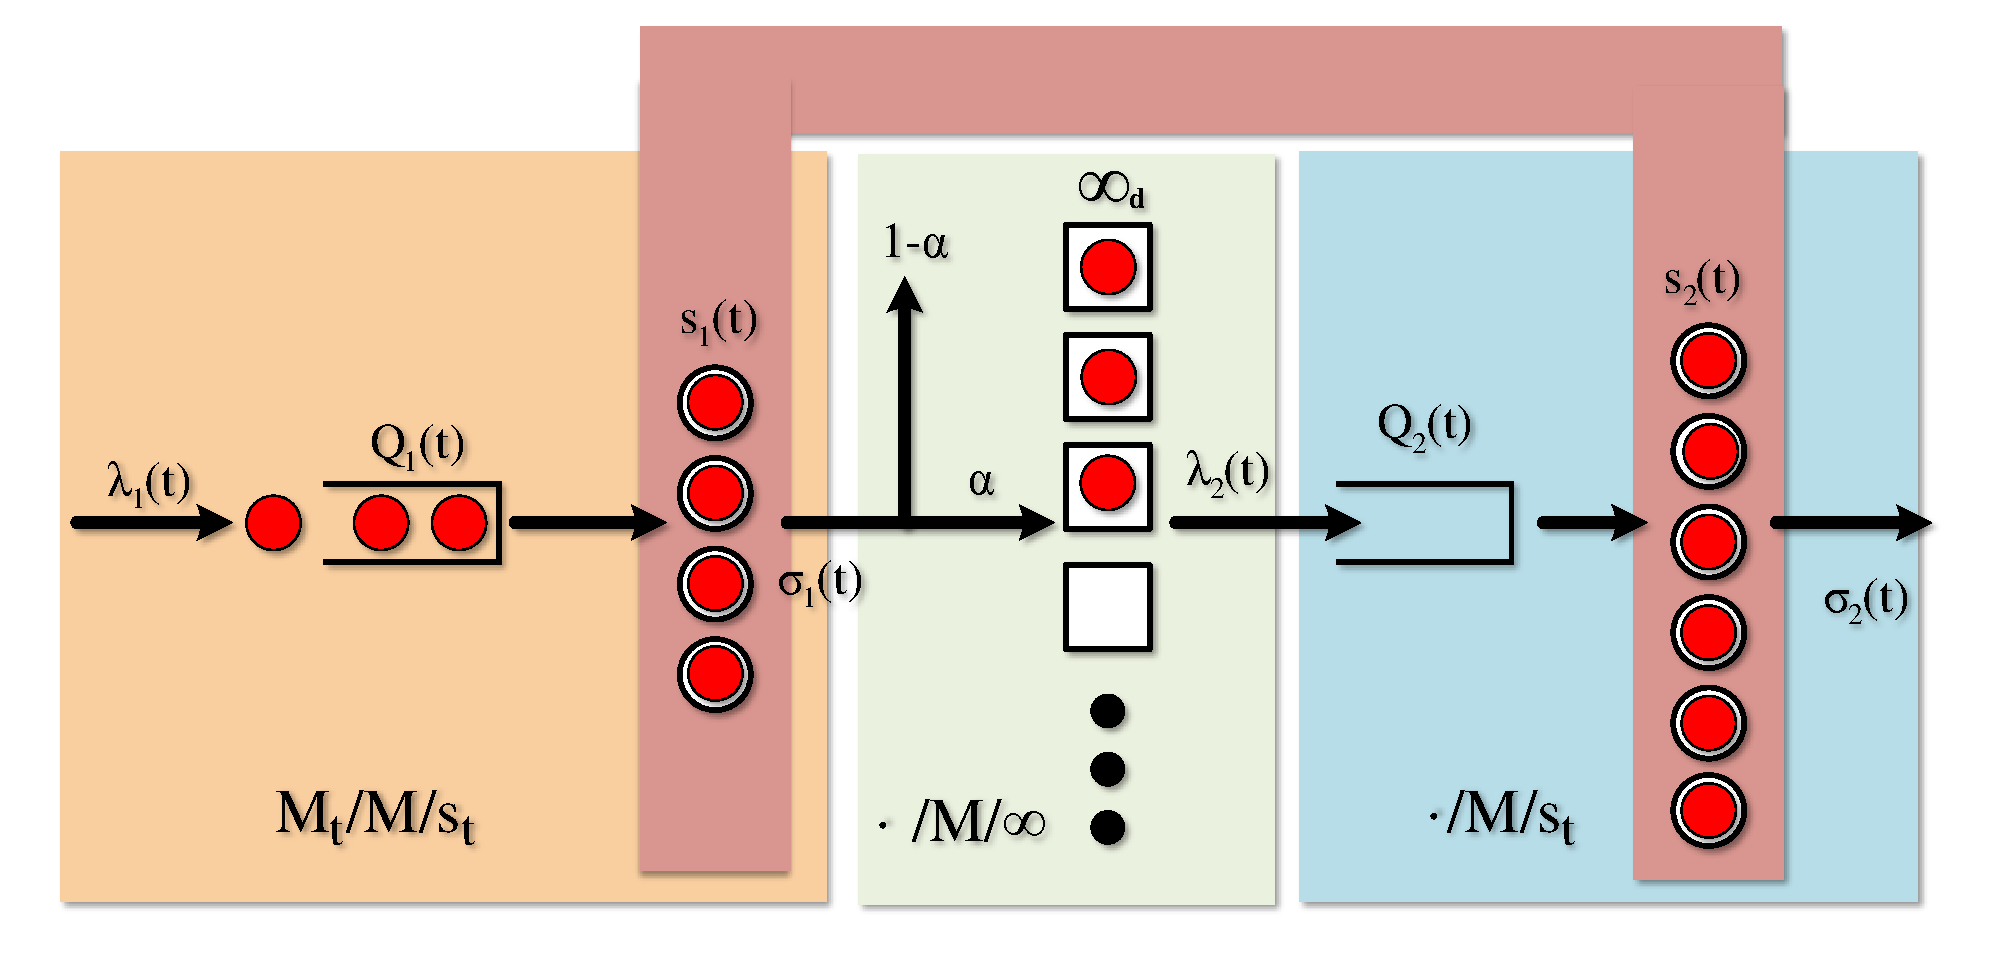
\includegraphics[width=0.9\linewidth]{./Figures/multiserver_avi.pdf}
% 	\caption{A stochastic tandem queue: two service station with intermediate delay}
	\label{fig:multiserver}
    \end{figure}
\begin{itemize}
    \item Shared service resources at phase (station) 1 and 2
    \item No control on the intermediate delay
    \item Time-varying arrival rate
\end{itemize}
\end{frame}

\begin{frame}{System Dynamics}

\begin{itemize}
	\item $X_i(t)$: the total number of patients at station $i$
	\item $s_i(t)$: the total number of nurses at station $i$
	\item $Q_i(t) \equiv (X_i(t) - s_i(t))^+$: the number of waiting patients at station $i$
	\item $\sigma_i(t)=\mu_i({X}_i(t) \wedge {s}_i(t))$: the departure rate at station $i$
\end{itemize}


\footnotesize
\begin{align}
{X}_1(t) &= {X}_1(0)+{N}_1\left(\int_{0}^{t}\lambda_1(u)du \right)-  {N}_{1d}^1\left(\alpha\mu_1\int_{0}^{t}  \left( {X}_1(u) \wedge {s}_1(u) \right)  du \right) \nonumber\\
&\qquad - {N}^2_{1d}\left((1-\alpha)\mu_1\int_{0}^{t} \left( {X}_1(u) \wedge {s}_1(u) \right)  du \right),\label{ch3:key1}\\
{X}_d(t) &= {X}_d(0)+{N}^1_{1d}\left(\alpha\mu_1\int_{0}^t{X}_1(u) \wedge {s}_1(u)du \right) - {N}_{d2}\left(\mu_d\int_{0}^t {X}_d(u)du \right),\\
{X}_2(t)&={X}_2(0)+{N}_{d2}\left(\mu_d\int_{0}^t {X}_d(u)du \right)-{N}_{20}\left(\int_{0}^{t}\mu_2 \left( {X}_2(u) \wedge {s}_2(u) \right) du \right)\label{ch3:key2},
\end{align}
\normalsize
where $ N_k $'s are all rate 1 Poisson process.
\end{frame}

\begin{frame}{A Stochastic Control Problem}
\begin{itemize}
    \item Performance function: $\int_{0}^{T}c_1Q_1(t) + c_2Q_2(t) dt $
	\item A stochastic control problem:
	\begin{align*}
	\min\limits_{s_1(t),s_2(t)}&\mathcal{R}(s_1(t),s_2(t) \equiv \mathbb{E}\left[\int_{0}^{T}\underbrace{ c_1Q_1(t) + c_2Q_2(t)  }_{\text{holding cost of waiting customers}}dt\right]\\
	s.t.&\quad \eqref{ch3:key1} - \eqref{ch3:key2},\\
	&\quad s_1(t)+s_2(t)\leq C(t),\\
	&\quad t\in[0,T].
	\end{align*}where $ C(t) $ is the total number of available servers.\medskip
	\item This stochastic programming problem is generally difficult to solve.
	\item MDP could be a workaround but multi-dimension MDP is not easy to analyze. See \cite{ahn2002optimal}.
	   % \begin{itemize}
	   %     \item High dimension
	   %     \item 
	   % \end{itemize}
\end{itemize}
\end{frame}

\begin{frame}{An Approximation: Fluid Model}
    % \setbeamertemplate{enumerate items}[square]
\begin{enumerate}
%	\item[1.] Model a service network as a queueing network.\medskip 
	\item \textit{Many-server} time-varying fluid approximation: \cite{liu2012g,mandelbaum1998strong} \item Increase \textcolor{Cyan}{arrival rate} and \textcolor{Cyan}{number of servers}
% 	\textcolor{Cyan}{Apply performance approximation} and construct an optimal control problem\smallskip

	%	\item Solve the related control problem and design control policy for the original system
\end{enumerate}
\vspace*{-0.2in}
\begin{figure}[ht]
	\centering
	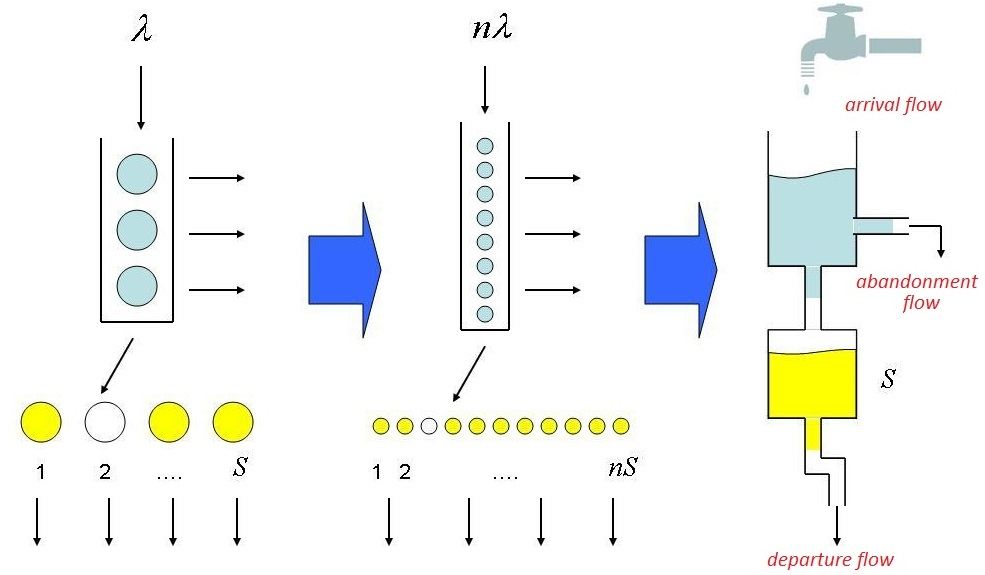
\includegraphics[width=0.65\textwidth]{./Figures/fluid3}
\end{figure}
\vspace*{-0.1in}
Let $ Q^n(t) $ be the queue length of a system with scale\footnote{A single number index for the size of a system: average numbers of arrival} $ n $ at time $ t $. 
\begin{itemize}
	\item A first-order approx.: $ Q^n(t)\approx n\bar{Q}(t) $
	\item $ \bar{Q}(t) $: deterministic, continuous-time function
\end{itemize}
\end{frame}

\begin{frame}{Apply Fluid Approximation}
\begin{itemize}
    \item Create a sequence of stochastic model indexed by total service capacity, which we denote as $n$
    \begin{equation}
        \begin{array}{c}
          Q_i^n(t),~ X_i^n(t),~ \lambda_n(t)=n\lambda(t),~ c_i^n=c_i,~ \mu_i^n=\mu_i,~ s_i^n(t)=ns_i(t)
        \end{array}
    \end{equation}
    \item Prelimit fluid-scaled process
        \begin{equation}
            \begin{array}{c}
                 \bar{Q}^n_i(t) = \dfrac{ Q_i^n(t)}{n}, \quad \bar{X}^n_i(t) = \dfrac{ X_i^n(t)}{n}
            \end{array}
        \end{equation}
        
    \item Convergence to continuous and deterministic fluid model
        \begin{equation}
            \begin{array}{c}
                  \bar{Q}^n_i(t)\rightarrow \bar{Q}_i(t), \quad \bar{X}^n_i(t)\rightarrow \bar{X}_i(t)
            \end{array}
        \end{equation}
    \item Fluid approximation
    \begin{align}
        \mathbb{E}[Q_i^n(t)]\approx n \bar{Q}_i(t), \quad\mathbb{E}[X_i^n(t)]\approx n \bar{X}_i(t)
    \end{align}
\end{itemize}
\end{frame}

\begin{frame}{An Asymptotic Framework: A Fluid Model}
Flow conservation gives the following:
\small
\begin{align}
\bar{X}_i(t) &= \bar{X}_i(0) + \int_0^t \left(\lambda_i(y) - \mu_i \left( \bar{X}_i(y)\land \bar{s}_i(y) \right)  \right) dy, \label{fluid:equ1} \\
\bar{X}_d(t) &= \bar{X}_d(0)+ \alpha\mu_1\int_{0}^t \bar{X}_1(y) \wedge {s}_1(y)dy - \mu_d\int_{0}^t \bar{X}_d(y)dy,\label{fluid:orbit}\\
\lambda_2(t) &= \int_0^t \alpha\lambda_d(t-y)f_d(y)dy = \int_0^t \alpha\mu_1\left( \bar{X}_1(t-y)\land \bar{s}_1(t-y) \right)dy.\label{fluid:equ2}
\end{align}
\normalsize 

\begin{theorem}[Convergence to fluid model]\label{thm:weak_convergence}
	Assume $\mathbb{E}[|\bar{X}_i^n(0) - \bar{X}_i(0)| ] \rightarrow 0$ for some deterministic $\bar{X}_i(0)\geq 0$, where $i\in\{1,2,d\}$. Under the assumptions above, we have for $t\geq 0$
	\begin{align}
	\mathbb{E}\left( \sup\limits_{0\leq t\leq T}|\bar{X}^n_i(t) - \bar{X}_i(t) |  \right)\rightarrow 0, \quad as~n\rightarrow \infty.
	\end{align}	where $\bar{X}_i(t)$ follows the equalities \eqref{fluid:equ1} - \eqref{fluid:equ2}.\footnote{A possible choice of $ n $ is the maximum available number of servers.}
\end{theorem} 
\end{frame}

\begin{frame}{A Fluid-based Optimal Control Problem}

\small
\begin{equation*}
\begin{array}{clr}
\displaystyle \min\limits_{\{(\bar{s}_1(t),\bar{s}_2(t))\} } &  \displaystyle \mathcal{\bar{R}}=\sum_{i=1}^2\int_{0}^{T} c_i\left( \bar{X}_i(t) - \bar{s}_i(t)\right)^+dt  &\\ [10pt]
\displaystyle s.t. & & \quad \\
& \displaystyle \bar{X}_i(t) = \bar{X}_i(0) + \int_0^t \left(\lambda_i(y) - \mu_i \left( \bar{X}_i(y)\land \bar{s}_i(y) \right)  \right) dy &\quad  i=1,2\\ [12pt]
%	& \displaystyle \bar{Q}_i(t) = (\bar{X}_i(t) - \bar{s}_i(t))^+ &\quad  i=1,2 \\ [10pt]
%       	& \displaystyle \lambda_d(t) = \mu_1\left( \bar{X}_1(t)\land s_1(t) \right) &\\ [10pt]
& \displaystyle \lambda_2(t) =  \int_0^t \alpha\mu_1\left( \bar{X}_1(t-y)\land \bar{s}_1(t-y) \right)dF_d(y) &\\ [10pt]
& \displaystyle \bar{s}_1(t) + \bar{s}_2(t) \leq \bar{C}(t) &\\ [10pt]
%         & \displaystyle \bar{s}_1(t) + \bar{s}_2(t) +s_{idle}(t) =  \bar{C} &\\ [10pt]
\end{array}
\end{equation*}

\begin{itemize}
    \item We provide a theorem and numerical solution method to substantiate the effectiveness of FCP. 
\end{itemize}
\end{frame}

\begin{frame}{Asymptotic Optimality}
	\begin{theorem}[Asymptotic Optimality]\label{thm:asym_optimality}
	Let $ (\bar{s}_1, \bar{s}_2) $ be one feasible solution to the FCP and $\bar{V}$ be the objective function value. Similarly, let $ (\bar{s}_1^*, \bar{s}_2^*) $ be the optimal solution to the FCP, and let $ \bar{V}^* $ denote its optimal value. 		
	\begin{itemize}
		\item []	Then $ \{ (n\bar{s}^*_1, n\bar{s}^*_2);n\geq 1 \}$ is asymptotically optimal, i.e.,	\begin{equation}\label{thm:ao_part1}
		\lim_{n\rightarrow\infty} \bar{\mathcal{R}}^n(n\bar{s}^*_1, n\bar{s}^*_2) = \bar{V}^*,
		\end{equation} and for any admissible sequence of $ (s_1^n, s_2^n) $
%		\item [$(ii)$] The asymptotic optimality is established by considering any admissible\footnote{If $ (s_1^n, s_2^n) $ is non-anticipative and the sum is bounded.} $ \{(s_1^n, s_2^n)\} $,		
		\begin{equation}\label{thm:ao_part2}
		\liminf_{n\rightarrow\infty} \bar{\mathcal{R}}^n(\bar{s}_1^n, \bar{s}_2^n) \geq \bar{V}^*.
		\end{equation}			
	\end{itemize}	
\end{theorem}
\end{frame}

\begin{frame}{A Discrete-time Solution Method}
\small
\begin{equation}\label{discrete:linearized}
\begin{array}{cl}
\displaystyle \min\limits_{\substack{ \{ (\bar{s}_{1,k},\bar{s}_{2,k},\bar{C});\\k = 1,\cdots,K \} } } &  \displaystyle \mathcal{\bar{R}}=\sum_{k=1}^K \left( c_1\bar{Q}_{1,n} + c_2\bar{Q}_{2,n} + c_w Y^-_{i,k} \right) \Delta t \\ [14pt]
%         \displaystyle s.t. & \displaystyle \bar{X}_{i,k} = \bar{X}_{i,0} + \sum_{l=0}^k \left(\lambda_{1,l} - \mu_i \bar{B}_{i,l}  \right) \Delta t \\ [14pt]
\displaystyle s.t. & \displaystyle \bar{X}_{i,k} - \bar{X}_{i,(k-1)} = \left( \lambda_{1,k} - \mu_i \bar{B}_{i,k}\right)\Delta t \\ [0pt]
%         & \displaystyle \bar{Q}_{i,k} = Y^+_{i,k}  \\ [0pt]
& \displaystyle \lambda_{2,k} =  \sum_{l=0}^k \alpha\mu_1\bar{B}_{1,k-l} \left( F_d((l+1)\Delta t) - F_d(l\Delta t) \right)  \\ [4pt]	
& \displaystyle \bar{B}_{i,k} \geq \bar{X}_{i,k} - \bar{Q}_{i,k} - Y^-_{i,k},\quad \bar{B}_{i,k} \geq \bar{s}_{i,k} - \bar{Q}_{i,k} - Y^-_{i,k} \\ [0pt]
%	& \displaystyle \bar{B}_{i,k} \geq \bar{s}_{i,k} - \bar{Q}_{i,k} - Y^-_{i,k} \\ [0pt]
& \displaystyle \bar{X}_{i,k} - \bar{s}_{i,k} = \bar{Q}_{i,k} - Y^-_{i,k},\quad \bar{B}_{i,k} \leq \bar{X}_{i,k}, \quad \bar{B}_{i,k} \leq \bar{s}_{i,k}\\ [0pt]
%	& \displaystyle \bar{B}_{i,k} \leq \bar{X}_{i,k}, \quad \bar{B}_{i,k} \leq \bar{s}_{i,k} \\ [0pt]
& \displaystyle \bar{s}_{1,k} + \bar{s}_{2,k} \leq \bar{C}_k \\ [0pt]
& \displaystyle \bar{Q}^+_{i,k} \geq 0,\quad \bar{X}^+_{i,k} \geq 0,\quad\bar{s}^+_{i,k} \geq 0 \\[0pt]
& \displaystyle \bar{B}_{i,k}\geq 0, \quad \lambda_{2,k} \geq 0,\quad Y^+_{i,k} \geq 0, \quad  Y^-_{i,k}\geq 0  \\[0pt]
& i=1,2\quad k=1,\cdots,K, \\
\end{array}
\end{equation}where $ \bar{B}_{i,k} $, $ Y^+_{i,k} $, $ Y^-_{i,k} $ are auxiliary variables.
\end{frame}

\begin{frame}{A Numerical Example}
	\begin{figure}[h!]
	\centering
	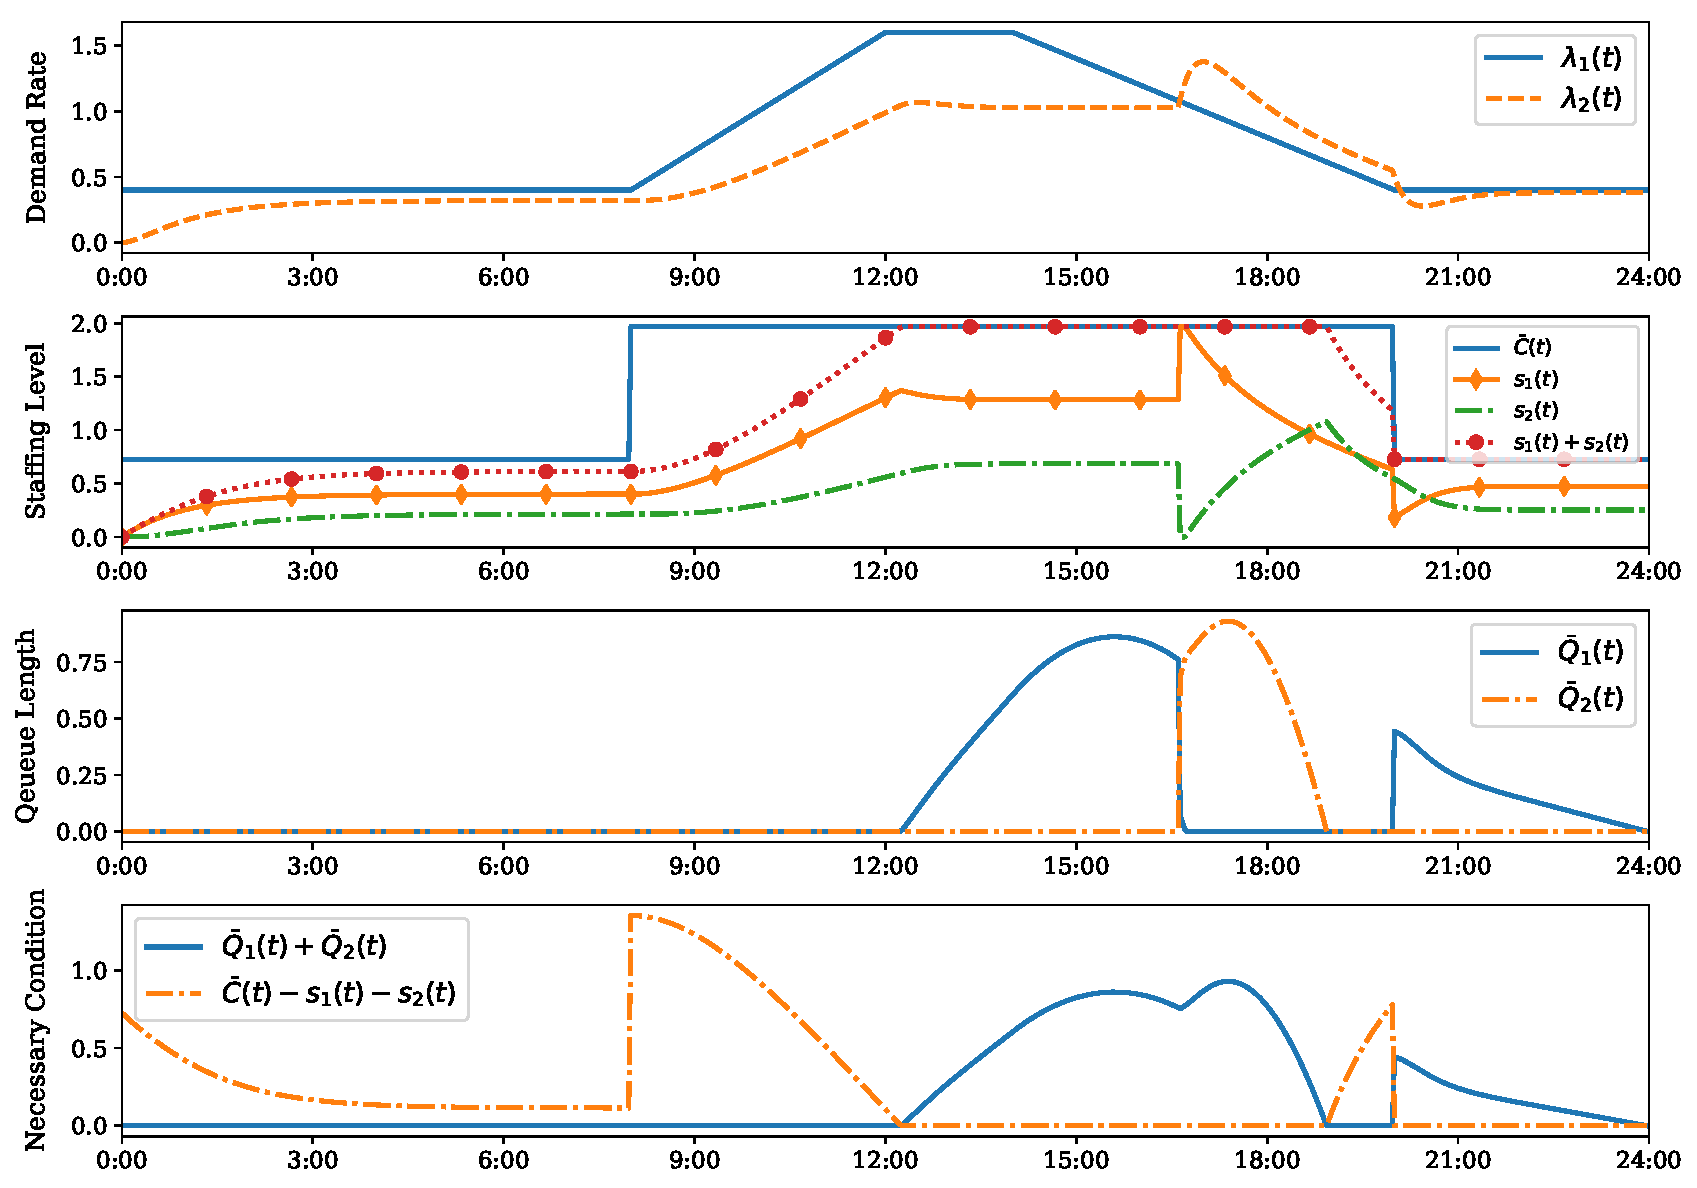
\includegraphics[width=0.8\textwidth]{./Figures/practical_exp}
%	\caption{A practical example: $ T=24$, $ \mu_1 = 1$, $ \mu_2=1.5$, $ \alpha= 0.8$, $ \mu_d=4$. The external patient arrival rate $ \lambda_1(t) $ is piece-wise linear. Shift switching times are $t_1 = 8$ and $t_2 = 20$. Cost coefficients: $ c_1=5 $, $ c_2 =3$, and $ c_s=13$. }
	\label{fig:practical_exp}
\end{figure}
\begin{itemize}
	\item Non-idling condition:
	$$(Q_1(t)+Q_2(t))(C-s_1(t) -s_2(t))=0.$$
\end{itemize}
\end{frame}

\begin{frame}{Structure Result: A Single-server Model}
    \begin{figure}[h!]
	\centering
	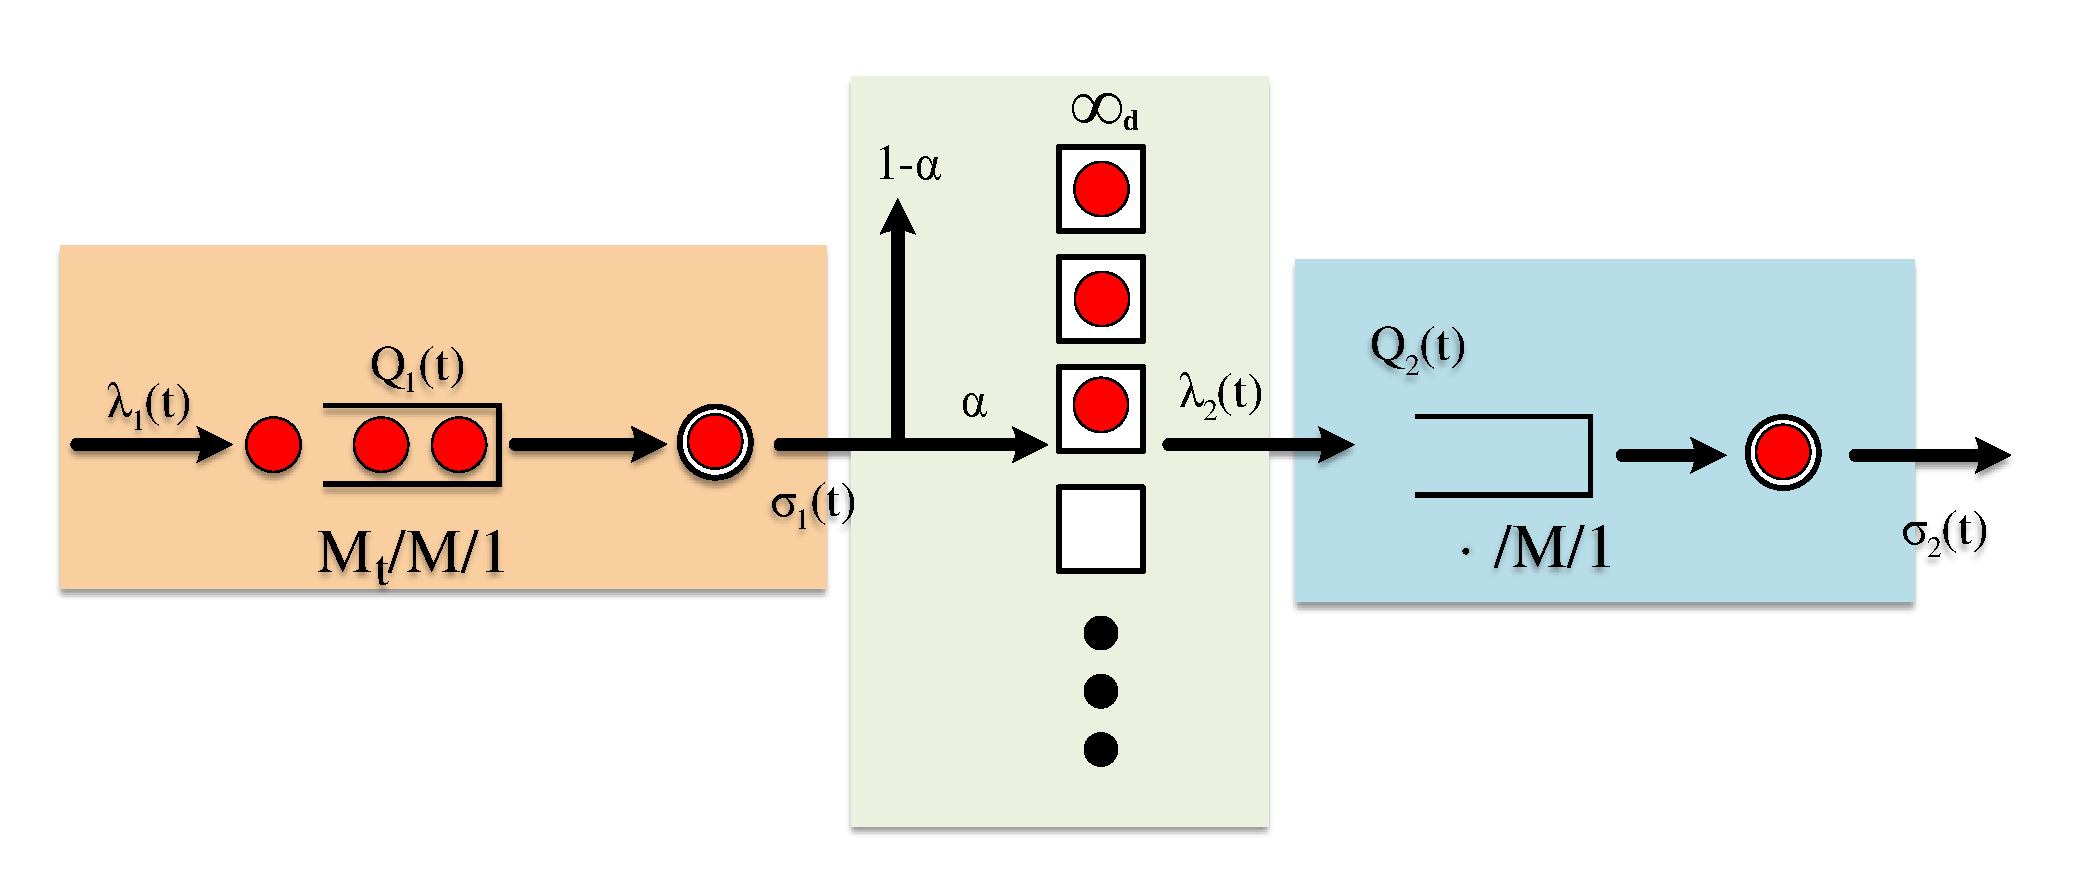
\includegraphics[width=0.8\textwidth]{./Figures/singleserver}
\end{figure}
\vspace{-0.2in}
% \begin{multicols}{2}
% \begin{itemize}
%     \item Use Pontryagin's Maximum Principle
%     \item Assume that both service stations are overloaded
% \end{itemize}
% \end{multicols}
% \begin{minipage}{.5\textwidth}
\begin{align*}
\min_{s_1,\ s_2}\quad & \int_{0}^T c_1x_1(t)+c_2x_2(t)dt \\
\text{s.t.}\quad &\dot{x}_1 = \lambda(t)-\mu_1s_1(t),\\
& \Dot{x}_d = \alpha\mu_1s_1(t)-\mu_dx_d(t),\\
& \Dot{x}_2 = \mu_dx_d(t)-\mu_2s_2(t),\\%& x_1(t) + x_2(t) \leq C \label{fcp:total_fluid}\\
& 0< s_1(t) + s_2(t) \leq 1,\\
& x_1(t) \geq 0,\ x_2(t) \geq 0.
\end{align*}
% \end{minipage}%
% \hfill
% \hfill
% \begin{minipage}{0.5\textwidth}
% \begin{itemize}
%     \item Use Pontryagin's Maximum Principle
%     \item Assume that both service stations are overloaded
% \end{itemize}
% \end{minipage}
\end{frame}

\begin{frame}{Insights "$c\mu$" Rule}
% \begin{table}[h!]
% \centering
% \begin{tabular}{|c|c|}
% 	\toprule \hline
% 	Parameter region $ c_1/c_2 $&{\emph{Priority Station}} 	\\\hline
% 	$ c_1/c_2\geq \check{\alpha}+\mu_2/\mu_1 $&{1}\\\hline
% 	$ \mu_2/\mu_1+\hat{\alpha} \leq  c_1/c_2 <\check{\alpha}+\mu_2/\mu_1 $ & 1 \\ \hline
% 	$ \mu_2/\mu_1<c_1/c_2<\mu_2/\mu_1+\hat{\alpha} $ & $ 2\rightarrow1 $ at $ t=s $ solves \eqref{equ:switcingpoint}\\\hline
% 	$ c_1/c_2\leq\mu_2/\mu_1 $&2\\\bottomrule
% \end{tabular}
% \vspace{0.1in}
% \caption{Note that $ 0< \hat{\alpha} < \check{\alpha}<\alpha $}
% \label{table:}
% \end{table}
In the \textcolor{Cyan}{no delay case}:
\begin{align*}
    (c_1-\alpha c_2)\mu_1 \quad vs\quad \mu_2 c_2
\end{align*}
In the \textcolor{Cyan}{delay case}:
\begin{table}[h!]
\centering
\begin{tabular}{|c|c|}
	\toprule \hline
	Parameter region &{\emph{Priority Station}} 	\\\hline
	$(c_1- \check{\alpha} c_2)\mu_1  \geq c_2\mu_2$ &{1}\\\hline
	$(c_1-\check{\alpha}c_2)\mu_1 <c_2\mu_2 \leq  (c_1-\hat{\alpha}c_2)\mu_1 $ & 1 \\ \hline
	$ (c_1-\hat{\alpha}c_2)\mu_1<c_2\mu_2<c_1\mu_1$ & $ 2\rightarrow1 $ at $ t=s $ solves \eqref{equ:switcingpoint}\\\hline
	$ c_1\mu_1\leq c_2\mu_2$&2\\\bottomrule
\end{tabular}
\vspace{0.1in}
% \caption{Recall that $ 0< \hat{\alpha} < \check{\alpha}<\alpha $ and therefore $c_1>c_1-\hat{\alpha}c_2>c_1-\check{\alpha}c_2$.}
\label{table:}
\end{table}
\vspace{-0.2in}
\begin{gather*}
0< \hat{\alpha} < \check{\alpha}<\alpha\\
    \hat{\alpha}=\alpha(1-\dfrac{1-e^{-\mu_dT}}{\mu_d T}),\quad \check{\alpha}=\alpha(1-e^{-\mu_d T})
\end{gather*}
\vspace{-0.1in}
\small
\begin{equation}\label{equ:switcingpoint}
\begin{array}{l}
0=-\mu_1c_1(s-T)+\alpha\mu_1\left(\dfrac{c_2}{\mu_d}(1-e^{\mu_d(s-T)})+c_2(s-T)\right)+\mu_2c_2(s-T)
\end{array}
\end{equation}
\end{frame}

\begin{frame}{Insights "$c\mu$" Rule: Graph Representation}
    \begin{figure}
        \centering
        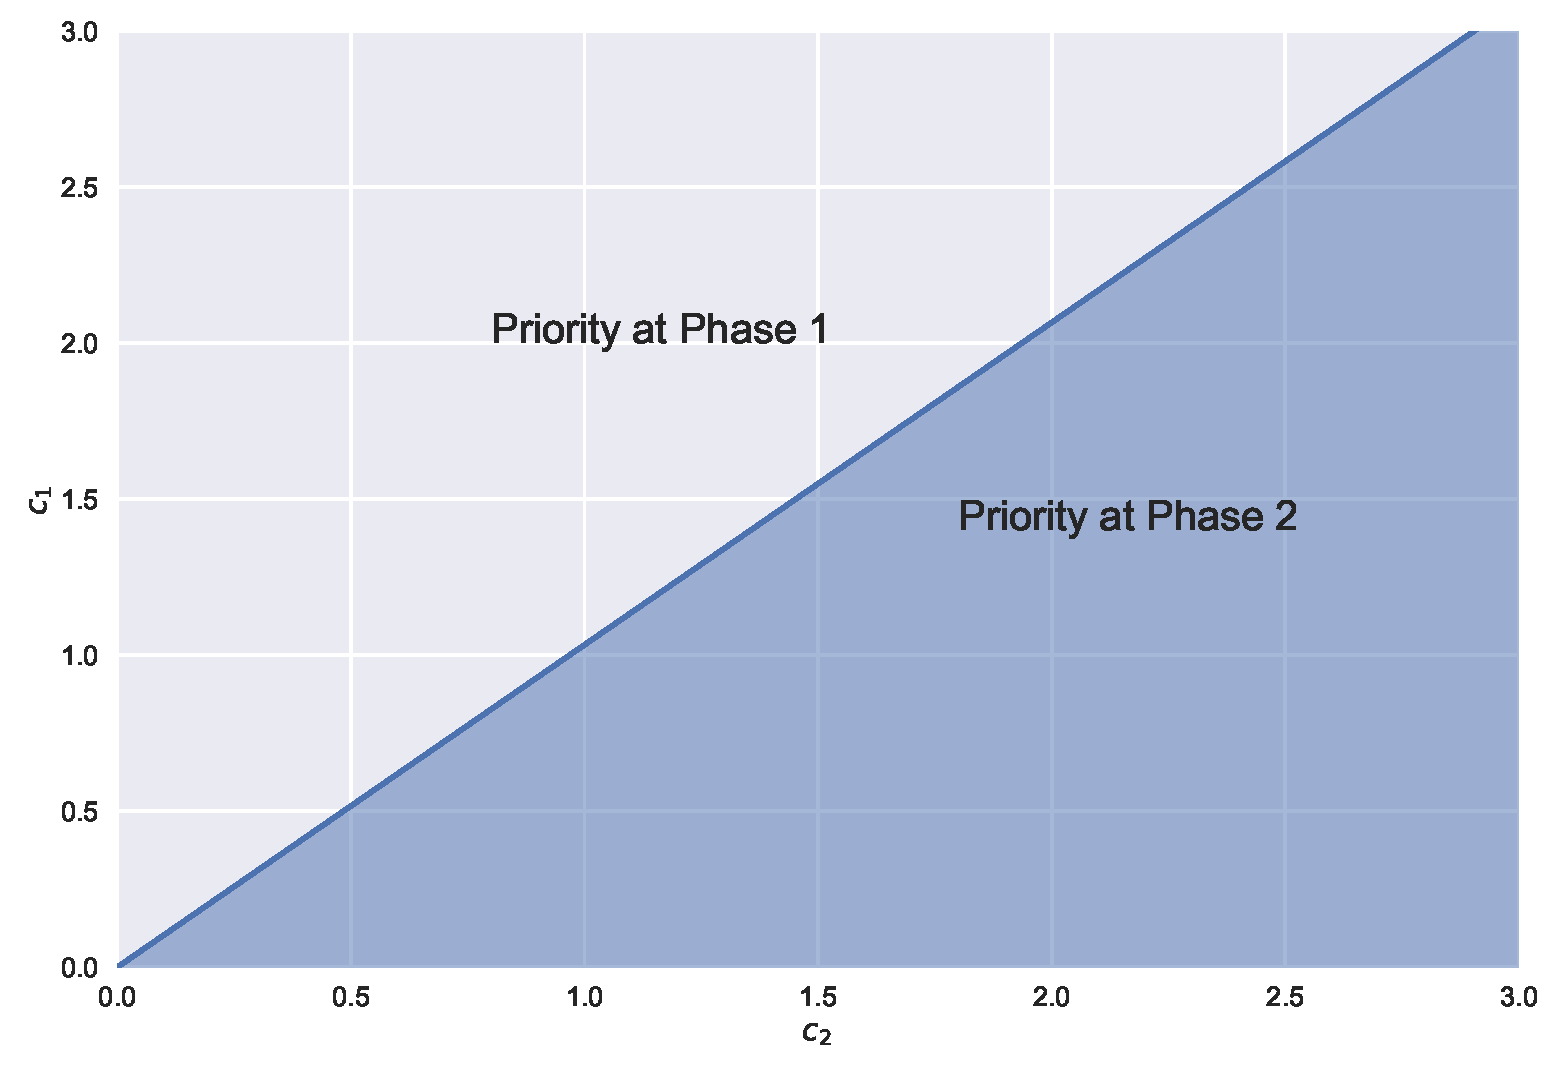
\includegraphics[width=0.9\textwidth]{Figures/nodelay}    
        % 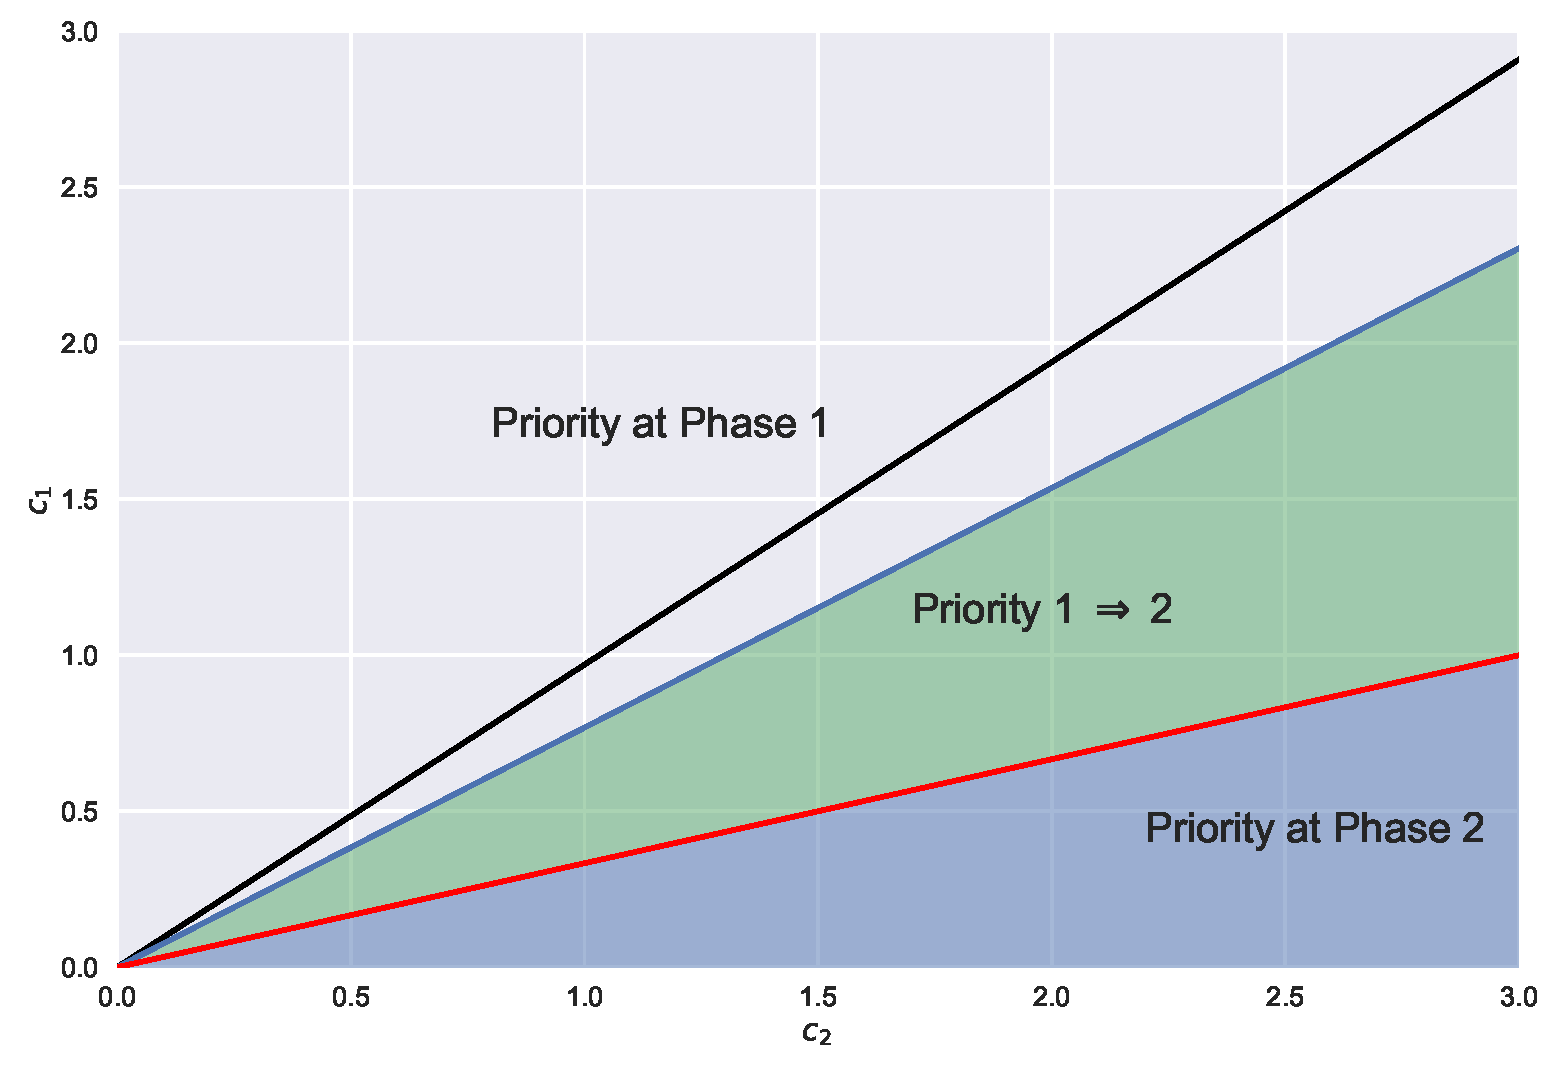
\includegraphics[width=0.5\textwidth]{Figures/withdelay}
        \caption{No delay}
        % \label{fig:my_label}
    \end{figure}
\end{frame}

\begin{frame}{Insights "$c\mu$" Rule: Graph Representation}
    \begin{figure}
        \centering
       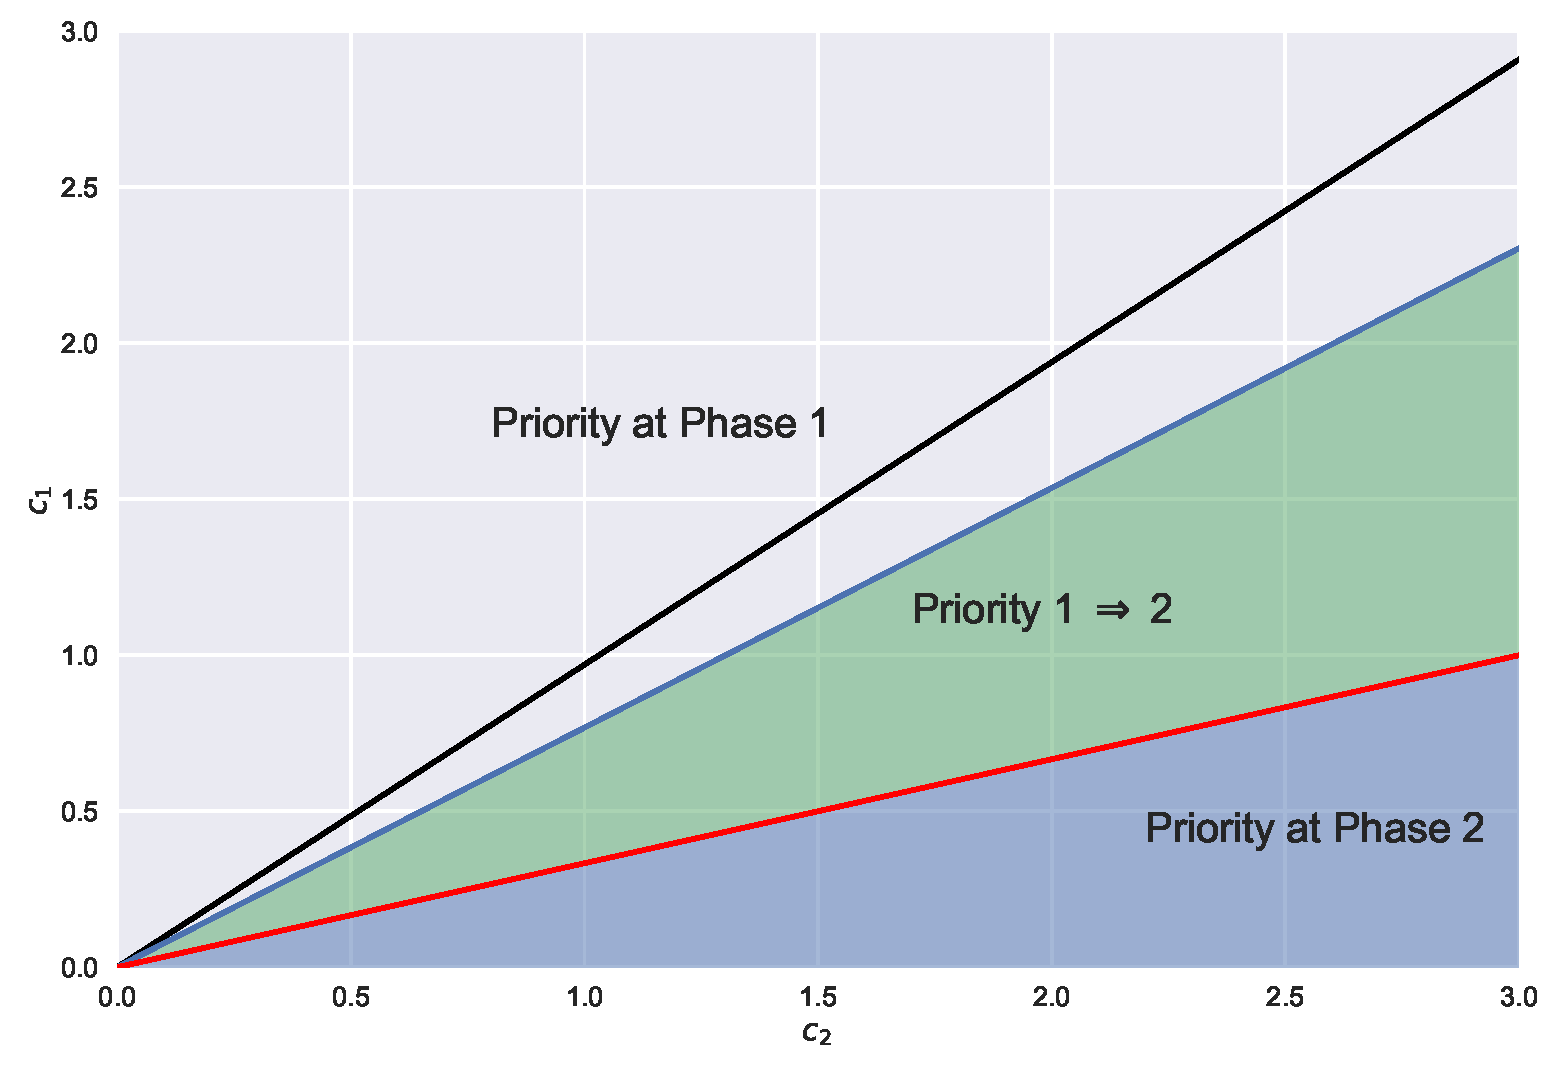
\includegraphics[width=0.9\textwidth]{Figures/withdelay}
        \caption{With delay}
        % \label{fig:my_label}
    \end{figure}
\end{frame}

\begin{frame}{References}
\bibliographystyle{plainnat}
\bibliography{mybibTandem} 
\end{frame}


\end{document}
